\documentclass[20pt]{beamer}
\usepackage[size=custom, height=80, width=100, scale=1.5]{beamerposter}
\usepackage{graphicx}
\usepackage{multicol}
% \usepackage{amsmath}
% \usepackage{amssymb}
\usepackage[numbers]{natbib}
\usepackage{soul}

\setulcolor{black}
\newcommand{\heading}[1]{\ul{\textbf{#1}} \\}
\bibliographystyle{plainnat}

% Theme settings
% \usetheme{ConfPoster} 
% \usecolortheme{dolphin}  % You can experiment with different color themes

% Title and Author Information
\title{Automatic Summarization of Long Documents}
\author{
  Naman Chhibbar\textsuperscript{\rm 1},
  Jugal Kalita\textsuperscript{\rm 2}
}
\institute{
  \textsuperscript{\rm 1}Indian Institute of Technology, Hyderabad \\
  \textsuperscript{\rm 2}University of Colorado, Colorado Springs \\
  \texttt{naman.iith@gmail.com, jkalita@uccs.edu}
}

\begin{document}
\begin{frame}[t]

% Title Block
\begin{columns}[t]
  \column{.15\textwidth}
    \begin{figure}[!h]
      \centering
      
\includegraphics[width=.6\textwidth]{images/iith.png}
    \end{figure}
  \column{.85\textwidth}
    \vspace{1cm}
    \begin{minipage}{\columnwidth}
      \centering
      \huge\textbf\inserttitle \\
      \large\textbf\insertauthor \\
      \large\insertinstitute
    \end{minipage}
\end{columns}
\vspace{1cm}

% Poster Content
\begin{columns}[t]

  \column{.33\textwidth}
  \begin{block}{Introduction}
    The rapid growth of online textual data has made \textbf{document summarization} essential for extracting relevant information efficiently.
    \textbf{Transformer models} have demonstrated remarkable capabilities in this domain, producing coherent and relevant summaries.
    However, \textbf{long document summarization remains a challenge} due to the \textbf{limited context size} of transformers, which stems from quadratic memory and computational complexity of the attention mechanism \cite{du2023improving}.
    This constraint makes it difficult to process extensive texts wherein summarization is crucial for reducing reading time and improving comprehension.
    We explore novel methods to overcome input size limitations in transformers \textbf{without modifying the model architecture}.
    These methods can be integrated into any existing summarization pipelines, maximizing an LLM’s ability to extract key information.
  \end{block}

  \begin{block}{Methodology}
    \heading{Central Truncation}
    In this method, we truncate the text from the middle; that is, we keep parts of the beginning and end of the document.
    This time-efficient method is an adaptation of \cite{worsham-kalita-2018-genre} and \cite{sun2019fine}, both of which pertain to long text classification.
    We introduce a new hyperparameter to control the fraction of the text to be taken from the head.

    \heading{Document Skimming}
    This method first segments the document and then uniformly samples the segments, meaning each segment has an equal probability of being sampled.
    This ensures that the model is exposed to all parts of the document while preserving efficiency.
    We also experiment with removing redundant segments before and after sampling to prevent the model from repeating itself.
    \begin{figure}[!h]
      \centering
      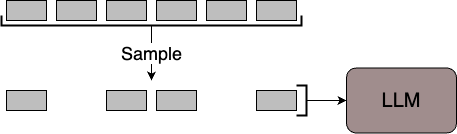
\includegraphics[width=\textwidth]{images/doc-skim.png}
      \caption{Document Skimming illustration. Grey blocks denote tokens in text.}
    \end{figure}
  \end{block}


  \column{.33\textwidth}
  \vspace{.8cm}
  \begin{minipage}{\columnwidth}
    \heading{Summarization with Keyword Extraction}
    This method is based on extracting keywords from the text to help choose the segments intelligently.
    We use LDA \cite{blei2003latent} with a single topic to extract topic words (keywords) from the text.
    These keywords are concatenated with space as a delimiter to form a single sentence.
    This sentence is compared against the segments using a sentence transformer using cosine similarity to gain scores for each segment.
    Segments with the highest scores are selected for summarization.
  \end{minipage}
  
  \begin{block}{Results}
    \begin{table}[!ht]
      \centering
      \small
    
      \begin{tabular}{c c c c c}
        \hline
        Model & R-1 & R-2 & R-L & BERTScore \\
        \hline
        BART /w Unlimiformer (1,024) & 53.4 & 22.5 & 22.5 & 66.0 \\
        PRIMERA w/ & 56.5 & 24.8 & 26.3 & 67.7 \\
        Unlimiformer (4,096) & & & & \\
        Hepos (10,240) & 51.34 & 19.09 & \textbf{48.73} & - \\
        PEGASUS-X /w Staggered & 60.3 & \textbf{30.0} & 31.5 & - \\
        Block-Local Attention (16k) & & & & \\
        LLaMA-7B /w Positional & 60.0 & 28.0 & 29.5 & - \\
        Interpolation (15k) & & & & \\
        \hline
        Summarization /w Extraction & \textbf{61.99} & 18.52 & 38.46 & \textbf{86.20} \\
        /w GPT-3.5 Turbo (4,096) & & & & \\
        Central truncation & 46.20 & 4.38 & 38.27 & 82.19 \\
        /w LongT5 (4,096) & & & & \\
        Skimming /w post-sampling & 46.76 & 4.56 & 39.61 & 81.96 \\
        removal /w LongT5 (4,096) & & & & \\
        \hline
      \end{tabular}
    
      % \caption{
      %   Automatic evaluation on GovReport dataset.
      %   The best metric in each category is highlighted in \textbf{bold}.
      % }
      \label{tab:govreport}
    \end{table}
    
    \begin{table}[!t]
      \centering
      \small
    
      \begin{tabular}{c c c c c}
        \hline
        Model & R-1 & R-2 & R-L & BERTScore \\
        \hline
        BigBird-Pegasus (16k) & \textbf{60.64} & \textbf{42.46} & \textbf{50.01} & - \\
        \hline
        Skimming w/ pre-sampling & 27.40 & 3.31 & 21.25 & \textbf{82.62} \\
        removal w/ GPT-3.5 Turbo (4,096) & & & & \\
        Central truncation & 27.77 & 3.09 & 20.56 & 82.57 \\
        w/ GPT-3.5 Turbo (4,096) & & & & \\
        Skimming w/ post-sampling & 26.16 & 2.13 & 20.21 & 82.40 \\
        removal w/ GPT-3.5 Turbo (4,096) & & & & \\
        \hline
      \end{tabular}
    
      % \caption{
      %   Automatic evaluation on BigPatent dataset.
      %   The best metric in each category is highlighted in \textbf{bold}.
      % }
      \label{tab:bigpatent}
    \end{table}
  \end{block}


  \column{.33\textwidth}
  \begin{block}{Conclusion}
    Summarize the key takeaways from your research. 
    Highlight the importance of your findings.
  \end{block}

  \begin{block}{References}
    \small\bibliography{anthology.bib}
  \end{block}

  \begin{block}{Acknowledgments}
    All work herein reported is supported by the National Science Foundation under Grant No. 2349452.
    Any opinion, finding, or conclusion in this study is that of the authors and does not necessarily reflect the views of the National Science Foundation.
  \end{block}
\end{columns}

\end{frame}
\end{document}
